%%%%%%%%%%%%%%%%%%%%%%%%%%%%%%%%%%%%%%%%%%%%%%%%%%%%%%%%%%%%%%%%%%%%%%%
% This document is based on the template: Large Colored Title Article %
%                                         Version 1.1 (25/11/12)      %
%                                                                     %
% The template was downloaded from: http://www.LaTeXTemplates.com     %
%                                                                     %
% Original author:                                                    %
% Frits Wenneker (http://www.howtotex.com)                            %
%                                                                     %
% License:                                                            %
% CC BY-NC-SA 3.0 (http://creativecommons.org/licenses/by-nc-sa/3.0/) %
%                                                                     %
% Author of this version:                                             %
% Laura M. Castro (http://www.madsgroup.org/staff/laura)              %
%                                                                     %
% Original licensing terms are maintained                             %
%%%%%%%%%%%%%%%%%%%%%%%%%%%%%%%%%%%%%%%%%%%%%%%%%%%%%%%%%%%%%%%%%%%%%%%

%----------------------------------------------------------------------------------------
%	PACKAGES AND OTHER DOCUMENT CONFIGURATIONS
%----------------------------------------------------------------------------------------

\documentclass[DIV=calc,paper=a4,fontsize=11pt,onecolumn]{scrartcl}	 % A4 paper and 11pt font size

\usepackage[galician]{babel} % Galician language/hyphenation
\usepackage[utf8]{inputenc}
\usepackage[protrusion=true,expansion=true]{microtype} % Better typography
\usepackage{amsmath,amsfonts,amsthm} % Math packages
\usepackage[svgnames]{xcolor} % Enabling colors by their 'svgnames'
\usepackage[hang,small,labelfont=bf,up,textfont=it,up]{caption} % Custom captions under/above floats in tables or figures
\usepackage{booktabs} % Horizontal rules in tables
\usepackage{fix-cm}	 % Custom font sizes - used for the initial letter in the document
\usepackage{graphicx}
\usepackage{float}
\usepackage{subfig}
\usepackage{sectsty} % Enables custom section titles
\usepackage{url}
\allsectionsfont{\usefont{OT1}{phv}{b}{n}} % Change the font of all section commands

\usepackage{fancyhdr} % Needed to define custom headers/footers
\pagestyle{fancy} % Enables the custom headers/footers
\usepackage{lastpage} % Used to determine the number of pages in the document (for "Page X of Total")

% Headers - all currently empty
\lhead{}
\chead{}
\rhead{}

% Footers
\lfoot{}
\cfoot{}
\rfoot{\footnotesize Páxina \thepage\ de \pageref{LastPage}} % "Page 1 of 2"

\renewcommand{\headrulewidth}{0.0pt} % No header rule
\renewcommand{\footrulewidth}{0.4pt} % Thin footer rule

\definecolor{UDC}{RGB}{206,0,124}
\definecolor{DarkUDC}{rgb}{0.75,0.75,0.75}
\definecolor{LightUDC}{RGB}{128,128,128}

\usepackage{lettrine} % Package to accentuate the first letter of the text
\newcommand{\initial}[1]{ % Defines the command and style for the first letter
\lettrine[lines=3,lhang=0.3,nindent=0em]{
\color{UDC}
{\textsf{#1}}}{}}

%----------------------------------------------------------------------------------------
%	TITLE SECTION
%----------------------------------------------------------------------------------------

\usepackage{titling} % Allows custom title configuration

\newcommand{\HorRule}{\color{UDC} \rule{\linewidth}{1pt}} % Defines the pink horizontal rule around the title

\pretitle{\vspace{-30pt} \begin{flushleft} \HorRule \fontsize{20}{20} \usefont{OT1}{phv}{b}{n} \color{DarkUDC} \selectfont} % Horizontal rule before the title

\title{Arquitecturas distribuidas} % Your article title

\posttitle{\par\end{flushleft}\vskip 0.5em} % Whitespace under the title

\preauthor{\begin{flushleft}\large \lineskip 0.5em \usefont{OT1}{phv}{b}{sl} \color{DarkUDC}} % Author font configuration

\author{Adrián Insua Yañez} % Your name

\postauthor{\footnotesize \usefont{OT1}{phv}{m}{sl} \color{Black} % Configuration for the institution name
{} Universidade da Coruña % Your institution

\par\end{flushleft}\HorRule} % Horizontal rule after the title

\date{Arquitectura Software -- Curso 2015/2016} % Add a date here if you would like one to appear underneath the title block

%----------------------------------------------------------------------------------------

\begin{document}

\maketitle % Print the title

\thispagestyle{fancy} % Enabling the custom headers/footers for the first page 

%----------------------------------------------------------------------------------------
%	ABSTRACT
%----------------------------------------------------------------------------------------

% The first character should be within \initial{}
\initial{E}\textbf{n este documento describiranse as carecteristicas das arquitecturas distribuidas emuladas mediante nodos Erlang.}

\vspace*{1cm}

\tableofcontents

\clearpage

%----------------------------------------------------------------------------------------
%	ARTICLE CONTENTS
%----------------------------------------------------------------------------------------

\section{Arquitectura cliente servidor}

\subsection{Vista estática}
\begin{figure}[h]
\centering
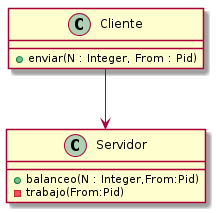
\includegraphics[width = 0.5\textwidth]{./figuras/estaticoCS.png}
\caption{Diagrama de modulos.}
\label{fig:estCS}
\end{figure}
\newpage
\subsection{Vista dinámica}

Como vemos na figura \ref{fig:dinCS} o cliente encargase da comunicación co servidor, e o modulo de servidor primeiro ocuparase do balanceo e despois cada un dos servidores ofrecerá un servizo distinto dende a sua función de traballo, e avisará o servidor de balanceo de que rematou.
\begin{figure}[!h]
\centering
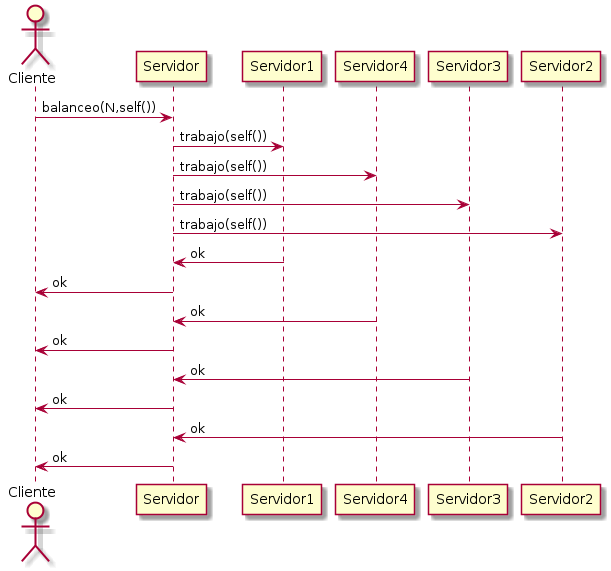
\includegraphics[width = 0.5\textwidth]{./figuras/dinamicoCS.png}
\caption{Vista Dinámica.}
\label{fig:dinCS}
\end{figure}

\newpage
\subsection{Vista despregue}

O grupo de servizos representase mediante un cartafol, con esto querese decir que pode haber 3 ou mais.
\begin{figure}[]
\centering
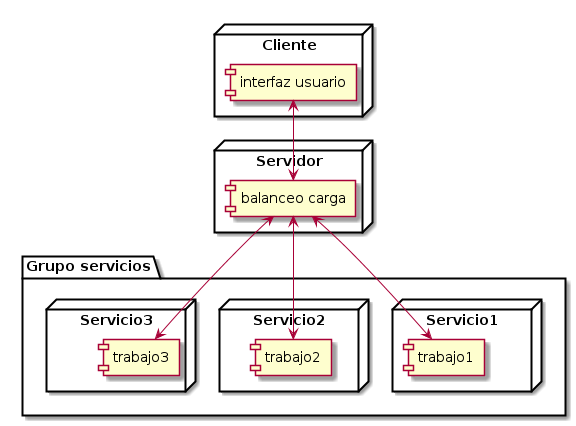
\includegraphics[width = 0.5\textwidth]{./figuras/despCS.png}
\caption{Vista Despregue.}
\label{fig:despCS}
\end{figure}
\subsection{Tempo}
O tempo acadado na realización de 500 probas nesta arquitectura foi de 202.89

\newpage
\section{Arquitectura mestre-escravo}

\subsection{Vista estática}
\begin{figure}[h]
\centering
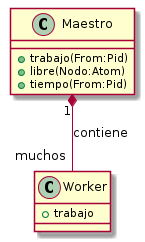
\includegraphics[width = 0.5\textwidth]{./figuras/estaticoMS.png}
\caption{Diagrama de modulos.}
\label{fig:estMS}
\end{figure}

\newpage
\subsection{Vista dinámica}
O que sucede na fig. \ref{fig:dinMS} podese explicar dicindo que o mentre envía traballo os traballadores indistintamente, e cando estes rematan devolvenlle o mestre unha mensaxe "libre" que os volve a habilitar.
Si se da o caso de que o mestre quere enviar traballo pero todos os traballadores estan ocupados, quedase esperando ata recibir a mensaxe "libre"

Os mensaxes de peticion de tempo incluense para entender o funcionamento da práctica xa que estas son as peticións que se lle fan o servidor para determinar si se remataran de procesar todos os traballos.
\begin{figure}[!h]
\centering
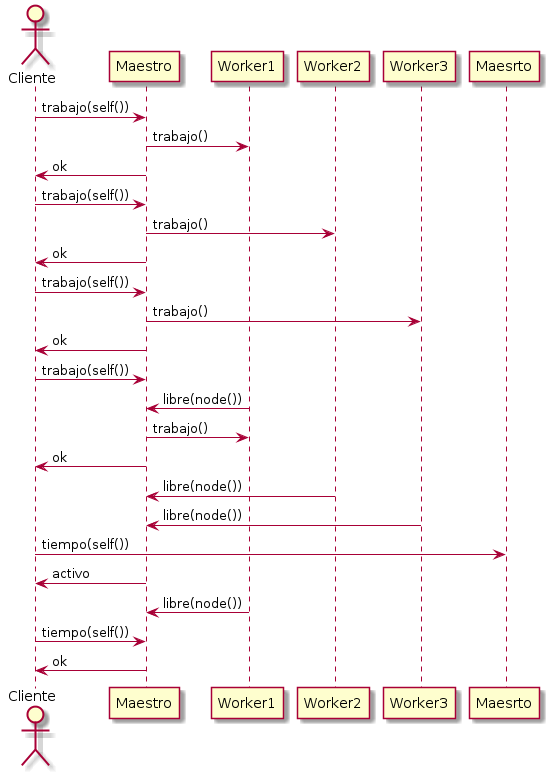
\includegraphics[width = 0.5\textwidth]{./figuras/dinamicoMS.png}
\caption{Vista Dinámica.}
\label{fig:dinMS}
\end{figure}

\newpage
\subsection{Vista despregue}
A representación e a mesma que a empregada na seccion anterior.
\begin{figure}[!h]
\centering
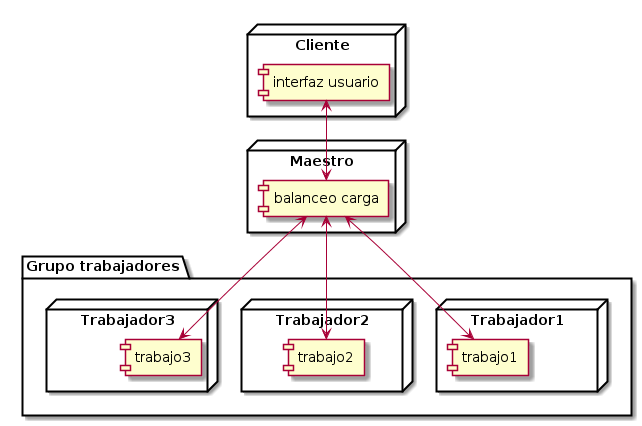
\includegraphics[width = 0.5\textwidth]{./figuras/despMS.png}
\caption{Vista Despregue.}
\label{fig:despMS}
\end{figure}
\subsection{Tempo}
O tempo acadado na realización de 500 probas nesta arquitectura foi de 64.584

\newpage
\section{Arquitectura P2P}

\subsection{Vista estática}
\begin{figure}[h]
\centering
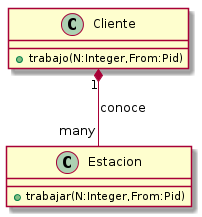
\includegraphics[width = 0.5\textwidth]{./figuras/estaticop2p.png}
\caption{Diagrama de modulos.}
\label{fig:estp2p}
\end{figure}

\newpage
\subsection{Vista dinámica}
Neste proceso o nodo peer pode decidir si quere realizar o traballo ou pasarllo a outro nodo
\begin{figure}[!h]
\centering
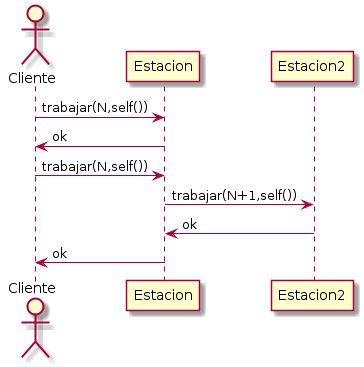
\includegraphics[width = 0.5\textwidth]{./figuras/dinamicop2p.png}
\caption{Vista Dinámica.}
\label{fig:dinp2p}
\end{figure}

\newpage
\subsection{Vista despregue}
En esta figura pretendese amosar que a comunicación e de todos a todo, é dicir un cliente pódese comunicar con calquer peer, e os peers entre eles tamén
\begin{figure}[!h]
\centering
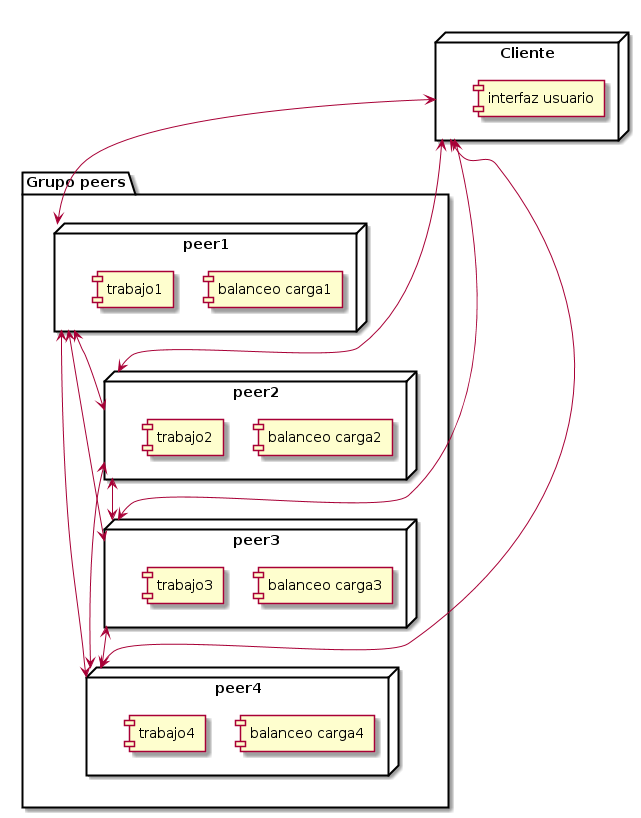
\includegraphics[width = 0.5\textwidth]{./figuras/despp2p.png}
\caption{Vista Despregue.}
\label{fig:despp2p}
\end{figure}
\subsection{Tempo}
O tempo acadado na realización de 500 probas nesta arquitectura foi de 308.3
\newpage
\section{Tempos}
\subsection{Táboa de resultados}

\begin{table}[]
\centering
\caption{My caption}
\label{my-label}
\begin{tabular}{lclll}
Arq. & \multicolumn{4}{c}{Tiempo} \\
C.S  & \multicolumn{4}{c}{202.89} \\
M.S  & \multicolumn{4}{c}{64.584} \\
P2P  & \multicolumn{4}{c}{308.3}      

Podemos obserbar no cadro \ref{my-label} que a arquitectura máis rápida é a m.s ainda que os datos non son fiables xa que se perde parte da capacidade de paralelización das arquitecturas na emulación.

A arquitectura de cliente servidor a pesar de perder un nodo de traballo para convertilo en balanceador amósa un tempo máis baixo que a arquitectura p2p, que pode ser que perda moito tempo debido a lóxica aplicada para decidir entre mover a carga de traballo a outro peer ou realizala el mesmo.
\end{tabular}
\end{table}
\end{document}
